\chapter{Comparação entre Métodos}
\label{cht:grupos}

Anteriormente foi feito um estudo sobre os métodos Ágil mais usados hoje em dia. No entanto, é necessário comparar os vários métodos por forma a podermos tirar conclusões e enquadrar estes métodos nos vários quadrantes, segundo as características próprias de cada um.
É normal não usar a mesma abordagem para um projeto onde é necessário criar apenas uma página web ou uma peça de software para um satélite da NASA. É também normal não usar a mesma abordagem com uma equipa de seis pessoas, do que com uma de sessenta pessoas ou até mesmo seiscentas pessoas. Diferentes situações exigem abordagens diferentes.
É fácil entender que é necessário alinhar a nossa abordagem mediante as variáveis do projeto em questão, e é por isso necessário não só dividir os vários métodos (tradicionais e Ágil) em várias categorias. 

\subsection{A necessidade de flexibilidade}

Para se ser bem sucedido no desenvolvimento de um software é necessário ser flexível na escolha do método utilizado. Existindo várias razões pelas quais é importante fazer:

\begin{itemize}
    \item \textbf{Diferentes tecnologias requerem diferentes técnicas} - Por exemplo, métodos orientados a objetos servem melhor projetos que usam tecnologias orientadas a objetos e métodos orientados aos dados servem melhor aplicações orientadas aos dados.
    \item \textbf{Cada pessoa é única} - Cada constituinte da equipa tem um background diferente, preferências de trabalho diferentes e diferentes gostos. Um método que sirva bem uma equipa, pode não resultar bem noutra equipa.
    \item \textbf{Cada equipa é única} - As equipas são feitas por pessoas, e como as pessoas são únicas a união destas pessoas torna-se também única. É importante adaptar o método de trabalho à equipa.
    \item \textbf{As necessidades exteriores podem variar} - Por exemplo, um projeto pode estar sujeito a regulamentações governamentais, ou pode estar sujeito a restrições de fornecedores ou até mesmo a desenvolvimento de terceiros. É importante também adaptar o método de trabalho para incorporar fatores exteriores.
    \item \textbf{As categorias dos projetos variam} - Diferentes tipos de projetos requerem diferentes abordagens porque cada categoria tem as suas prioridades e objetivos.
    \item \textbf{As categorias dos métodos variam} - Cada método Ágil tem as suas vantagens e desvantagens.
\end{itemize}

\subsection{As categorias dos métodos}

Os métodos de desenvolvimento podem ser separados em quatro categorias distintas:

\begin{itemize}
    \item \textbf{Code and Fix} - Abordagem conhecida também como "hacking". É por norma uma abordagem caótica e muitas vezes não planeada, ou quando planeada o plano é rapidamente abandonado. As estimativas e cronogramas, quando feitos, raramente são cumpridos na prática.
    \item \textbf{Rigoroso} - Os projetos de software nesta categoria são bem definidos e geralmente incluem procedimentos detalhados que os programadores devem seguir com bastante rigor. Por exemplo, os requisitos são identificados, revistos e aceites. O design do sistema é feito, revisto e aceite. Há espaço para feedback entre as fases, embora esse feedback seja fornecido por meio de um procedimento bem estruturado e as alterações revistas e aceites. Os sistemas são entregues de forma incremental.
    \item \textbf{Iterativo Rigoroso} - Os processos de software nesta categoria são bem definidos e geralmente incluem procedimentos detalhados que os programadores devem aplicar de maneira iterativa. Por exemplo, os requisitos do projeto podem ser definidos inicialmente em alto nível, com os detalhes posteriormente detalhados conforme necessário. O software é entregue numa base incremental após curtos ciclos de lançamento.
    \item \textbf{Ágil} - Abordagem para o desenvolvimento de software orientada para pessoas, que permite que respondam efetivamente às mudanças e que resulta na criação de sistemas de trabalho que atendam às necessidades dos stakeholders. Os processos de software nesta categoria são definidos a alto nível, geralmente apresentados como uma coleção de práticas ou filosofias. Os principais métodos Ágil foram já identificados e descritos no capítulo anterior.
\end{itemize}

Cada categoria apela a uma mentalidade diferente. Por exemplo, os métodos Code and Fix são mais apropriados para programadores independentes. Os métodos Rigorosos são apropriados para equipas que querem ter uma abordagem inicial simples, geralmente em indústrias muito regulamentadas e burocráticas. Os métodos Rigorosos Iterativos funcionam bem em ambientes que são propensos a burocracia, mas com abertura suficiente para práticas arriscadas promovidas pelo desenvolvimento iterativo. Por fim, os métodos Ágil são uma abordagem nova e que normalmente permite ter em conta todos os stakeholders do projeto.

\subsection{Comparação entre métodos}

No gráfico em baixo poderemos ver a comparação entre os vários métodos, tendo em conta a adaptação a cada projeto (de ad-hoc a prescriptive) e o tamanho do ciclo do projeto (de full lifecycle a partial methodology), ou seja, se acompanha toda a vida do projeto ou se será necessário adotar um novo método mais tarde. 

\begin{figure}[H]
    \centering
    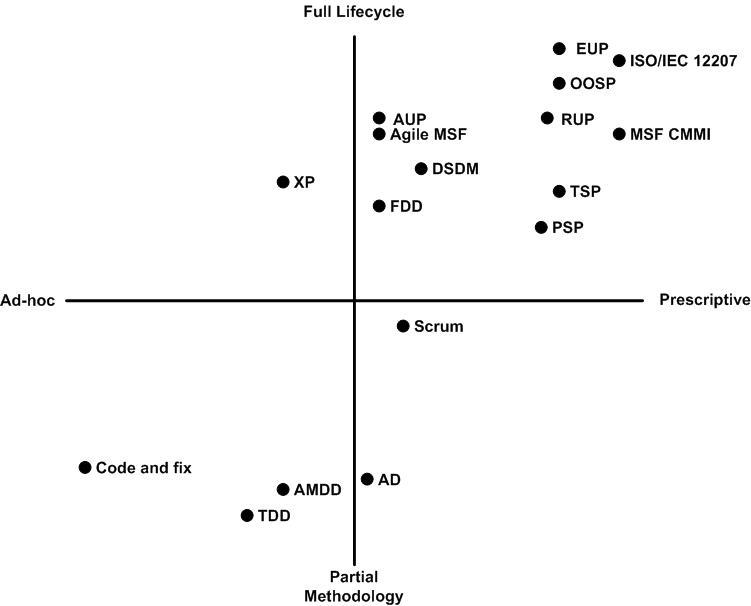
\includegraphics[scale=0.5]{Imagens/processComparisons.jpg}
    \caption{Comparação dos vários métodos}
    \label{fig:compme}
\end{figure}


\subsection{A necessidade de usar mais do que um método}

Nesta comparação foram tidos em conta os vários métodos, mais tradicionais ou mais inovadores, já que nem todas as organizações estão pré-dispostas e têm as características necessárias para adotar uma metodologia Ágil na sua organização interna. O facto de termos tido em conta também os métodos mais tradicionais deve-se ao facto de os métodos Ágil não servirem tudo, nem serem apropriados para tudo, especialmente quando os projetos de software podem variar tanto. É necessário por isso ter uma mente aberta e escolher o método mais apropriado. Nos capítulos seguintes tenta-se criar um método de diagnóstico para ser usado no início do projeto com o objetivo de tirar conclusões iniciais sobre a utilização ou não de um método Ágil.
\\É possível, numa mesma organização, adotar e suportar vários métodos dos descritos anteriormente, tendo, no entanto, em conta o seguinte:

\begin{enumerate}
    \item Não variar muito a quantidade de métodos e aplicar apenas um pequeno conjunto que sirvam a grande maioria dos projetos desenvolvidos.
    \item Não basta adotar o método, terá que haver um esforço inicial de trabalhar e modificar o método para se moldar à equipa que o vai usar.
    \item Definir objetivos em comum a todos os projetos, não procedimentos porque como já foi dito, cada projeto é um projeto.
    \item Definir bem a terminologia utilizada.
    \item Ser flexível.
    \item Priorizar requisitos e objetivos.
\end{enumerate}

De seguida apresenta-se uma tabela com as principais características dos métodos Ágil e que pode ser utilizada como ponto de partida para a escolha.

\begin{sidewaystable}[ht]
\centering
\label{grupos}
\resizebox{\textwidth}{!}{
\begin{tabular}{|l|l|l|l|l|l|l|}
\hline
Características/Método         & Extreme Programming                                                                                               & Scrum                                                               & Dynamic Systems Development Method                        & Test Driven Development                                                       & Adaptive Software Development                                                                         & Crystal Methods                                                           \\ \hline
Abordagem                      & Incrementos iterativos                                                                                            & Incrementos iterativos                                              & Iterativo                                                 & Iterativo                                                                     & Iterativo                                                                                             & Incremental                                                               \\ \hline
Tempo recomendado por iteração & Entre 1 e 6 semanas                                                                                               & Entre 2 a 4 semanas                                                 & 80\% da solução em 20\% do tempo total                    & Entre 2 dias e 2 semanas                                                      & Entre 4 e 8 semanas                                                                                   & Depende do método da família                                              \\ \hline
Equipa                         & Equipas pequenas (\textless{}20 pessoas)                                                                          & Aplicável a equipas de todos os tamanhos                            & Todos os tamanhos, equipa independente                    & Mais de uma equipa                                                            & Equipas pequenas (entre 5 a 9 membros)                                                                & Todos tamanho, depende do método da família                               \\ \hline
Comunicação da equipa          & Informal com reuniões diárias                                                                                     & Informal com reuniões diárias                                       & Baseado em documentação                                   & Baseado em documentação                                                       & Informal e pessoal                                                                                    & Informal e pessoal                                                        \\ \hline
Tamanho do Projeto             & Projetos pequenos                                                                                                 & Todos os tipos projetos                                             & Todos os tipos de projetos                                & Projetos complexos e com várias funcionalidades                               & Projetos pequenos                                                                                     & Todos os tipos de projeto                                                 \\ \hline
Envolvimento do cliente        & Envolvimento total do cliente                                                                                     & O próprio clientes faz parte da equipa                              & O cliente está presente no momento dos lançamentos        & O cliente recebe relatórios                                                   & O cliente está presente no momento dos lançamentos                                                    & O cliente está presente a cada incremento                                 \\ \hline
Documentação do projeto        & Documentação básico                                                                                               & Documentação básica                                                 & Documentação básica                                       & Documentação é importante                                                     & Documentação básica                                                                                   & Documentação básica                                                       \\ \hline
Especialidades                 & Testes, User Stories, Refatoração                                                                                 & Sprint, Sprint backlog, Scrum master                                & Prototipagem                                              & Diagramas UML                                                                 & Ciclo de aprendizagem                                                                                 & Vários métodos dentro da família adaptáveis a qualquer situação e projeto \\ \hline
Vantagens                      & Ambiente de trabalho aberto em que o cliente pode ser parte da equipa, práticas bem definidas, Feedback constante & Alto nível de comunicação e colaboração                             & Os requisitos são prioridade, gestão do projeto eficiente & Os relatórios e a documentação permitem efetuar várias tarefas ao mesmo tempo & É importante desenvolver os componentes de maior risco primeiro, o ciclo de aprendizagem é importante & A metodologia ajusta-se ao tipo de projeto e tamanho da equipa            \\ \hline
Desvantagens                   & Pouca documentação, pouca disciplina, a presença do cliente pode ser crucial                                      & Pouca documentação, o controlo sobre o projeto é por vezes reduzido & Documentação complexa                                     & Podem existir "pontos cegos"                                                  & Pouca documentação                                                                                    & A coordenação pode ser pouco eficiente entre as equipas                   \\ \hline
\end{tabular}}
\end{sidewaystable}